\documentclass[12pt]{article}
\usepackage{ficha}

\begin{document}

\ficha{Monotonia, Extremos e Otimização}

\instrucoes{Resolve os exercícios, apresentando um quadro de variação sempre que estudares a monotonia.}

\secao{Monotonia e Extremos}{Estuda a monotonia e determina os extremos relativos de cada função.}
\begin{exercicios}
  \item $f(x) = x^2 - 6x + 2$
  \item $f(x) = x^3 - 3x$
  \item $f(x) = -x^3 + 3x^2 + 9x$
  \item $f(x) = x^4 - 8x^2$
  \item $f(x) = 2x^3 - 9x^2 + 12x - 4$
  \item $f(x) = x + \dfrac{4}{x}$
  \item $f(x) = \dfrac{x}{x^2 + 1}$
  \item $f(x) = \dfrac{x^2}{x - 1}$
  \item $f(x) = x\sqrt{4 - x}$, \; em $]-\infty, 4]$
\end{exercicios}

\secao{Extremos Absolutos num Intervalo Fechado}{Determina o máximo e o mínimo absolutos de $f$ no intervalo indicado.}
\begin{exercicios}
  \item $f(x) = x^2 - 4x + 1$, \; em $[0, 5]$
  \item $f(x) = x^3 - 12x$, \; em $[-3, 3]$
  \item $f(x) = 2x^3 - 3x^2 - 12x$, \; em $[-2, 3]$
  \item $f(x) = \dfrac{x}{x^2 + 4}$, \; em $[0, 4]$
  \item $f(x) = x^4 - 2x^2 + 3$, \; em $[-2, 2]$
\end{exercicios}

\secao{Leitura do Gráfico da Derivada}{O gráfico representa a \textbf{derivada} $f'$ de uma função $f$, de domínio $\R$.}

\begin{center}
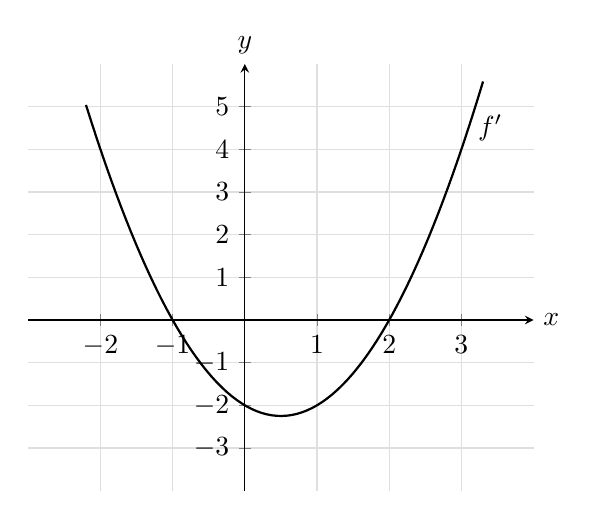
\begin{tikzpicture}
\begin{axis}[axis lines=middle, xmin=-3, xmax=4, ymin=-4, ymax=6, xtick={-2,...,3}, ytick={-3,...,5}, grid=both, grid style={gray!25}, width=8cm, height=7cm, xlabel=$x$, ylabel=$y$, every axis x label/.style={at={(ticklabel* cs:1)},anchor=west}, every axis y label/.style={at={(ticklabel* cs:1)},anchor=south}]
  \addplot[thick, domain=-2.2:3.3, samples=80] {(x+1)*(x-2)};
  \node at (axis cs:3.4,4.5) {$f'$};
\end{axis}
\end{tikzpicture}
\end{center}

\begin{exercicios}
  \item Indica os intervalos onde $f$ é crescente e onde é decrescente.
  \item Indica as abcissas dos extremos relativos de $f$ e classifica-os.
  \item Em que ponto a reta tangente ao gráfico de $f$ tem declive mínimo?
  \item Sabendo que $f'(x) = (x + 1)(x - 2)$ e $f(0) = 1$, determina $f(x)$.
\end{exercicios}

\secao{Problemas de Otimização}{Resolve, apresentando a função a otimizar e o seu domínio.}
\begin{exercicios}
  \item Determina dois números positivos cuja soma é 20 e cujo produto é máximo.
  \item Com 60\,m de rede, quer-se vedar um terreno retangular. Que dimensões dão área máxima?
  \item De uma folha quadrada de cartão com 30\,cm de lado cortam-se quadrados iguais nos cantos para fazer uma caixa sem tampa. Qual deve ser o lado dos quadrados cortados para o volume ser máximo?
  \item Uma lata cilíndrica deve ter 500\,cm$^3$ de volume. Determina o raio que minimiza a área total de material. (Arredonda às décimas.)
  \item Determina o ponto da reta $y = 2x + 1$ mais próximo do ponto $(4, 0)$.
  \item Um retângulo está inscrito na parábola $y = 12 - x^2$ e no eixo $Ox$, com dois vértices sobre o eixo. Determina as dimensões que maximizam a área.
  \item O lucro de uma empresa na venda de $x$ unidades é $L(x) = -0{,}02x^2 + 40x - 5\,000$ euros. Quantas unidades maximizam o lucro? Qual é o lucro máximo?
  \item Uma janela tem a forma de um retângulo encimado por um semicírculo. O perímetro é 8\,m. Que dimensões maximizam a área? (Arredonda às centésimas.)
\end{exercicios}

\secao{Desafios}{Resolve os problemas.}
\begin{exercicios}
  \item Determina $a$ e $b$ de modo que $f(x) = x^3 + ax^2 + b$ tenha um mínimo relativo no ponto $(2, -3)$.
  \item Mostra que, de todos os retângulos com o mesmo perímetro, o quadrado é o que tem maior área.
  \item Um homem está num barco a 3\,km da costa (ponto mais próximo $P$) e quer chegar a uma aldeia na costa a 6\,km de $P$. Rema a 4\,km/h e caminha a 5\,km/h. Onde deve desembarcar para chegar o mais depressa possível?
  \item Mostra que a equação $x^3 + 3x + 1 = 0$ tem exatamente uma solução real. (Usa a monotonia e o teorema de Bolzano.)
\end{exercicios}

\end{document}
